\chapter{\textit{Software} desenvolvido} \label{software}

Esse apêndice é manual de instalação e uso dos \textit{plugins} e \textit{jupyter notebooks} desenvolvidos. Os \textit{plugins} foram desenvolvidos para o software geostatístico \textit{AR2GeMS}. Recomenda-se a instalação e uso da suite de \textit{plugins} em uma versão do \textit{AR2GeMS} que inclua um interpretador python e a biblioteca \textit{ar2gas} embarcados (\textit{ar2gems-full-version-python3}).

A suite de \textit{plugins} pode ser acessada no repositório: \url{https://github.com/robertorolo/LPM-Geomod_Suite}. Para instá-la primeiro deve-se instalar as seguintes dependências \textit{ar2gas}, \textit{numpy}, \textit{math}, \textit{itertools}, \textit{scipy}, \textit{pyevtk}, \textit{sklearn}, \textit{pyevtk}. O reposítório conta com o arquivo \textit{install\underline{ }dependencies.py} ao copiar, colar e executar o conteúdo do arquivo no interpretador python embarcado no diretório do \textit{AR2GeMS} as dependências (com exceção do \textit{ar2gas} que não pode ser encontrado no repositório PyPI) são automaticamente instaladas.

Então, os arquivos (do repositório) da pasta \textit{ui} devem ser copiados e colados na pasta do \textit{AR2GeMS} plugins/Geostat, os arquivos da pasta \textit{py} devem ser copiados e colados na pasta do \textit{AR2GeMS} plugins/Geostat/python, finalmente, o arquivo \textit{helpers.py} deve ser copiado e colado na pasta \textit{Lib} do \textit{AR2GeMS}. Uma versão do \textit{AR2GeMS} com a suite previamente instalada pode ser solicitada ao autor dessa tese.

Caso a instalação tenha sido bem sucedida as \textit{plugins} serão mostrados no painel de algoritmos do \textit{software}, como mostrado na \autoref{algo_panel}.

\begin{figure}[H]
	\caption{\label{algo_panel} LPM-Geomod\underline{ }Suite no painel de algoritmos do \textit{AR2GeMS}.}
	\centering
		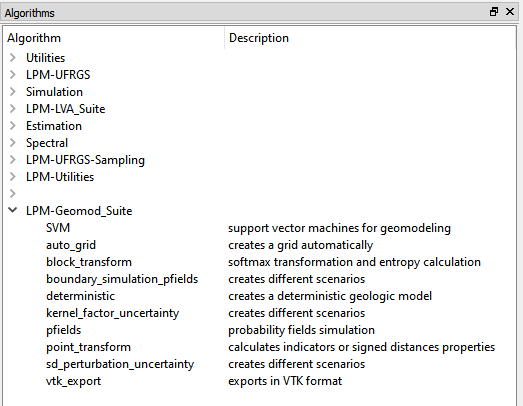
\includegraphics[width=0.6\textwidth]{apendice/imagens/algorithms.PNG}
\end{figure}

As próximas seções descrevem os diferentes \textit{plugins} e seus parâmtros.

\section{Transformações}

A suite traz ferramentas para transformar variáveis em pontos ou blocos.

\subsection{Em pontos}\label{pttrans_sec}

O \textit{plugin} \textit{point\underline{ }transform} (\autoref{pttrans}) recebe como \textit{input} a propriedade categórica que representa as diferentes litologias e faz a transformação em distâncias assinaladas ou indicadores. O \textit{output} são K propriedades, onde K é o número de litologias do banco de dados.

\begin{figure}[H]
	\caption{\label{pttrans}Interface do \textit{plugin} \textit{point\underline{ }transform}}
	\centering
		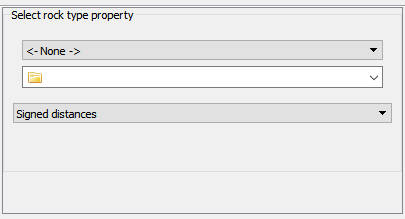
\includegraphics[width=0.6\textwidth]{apendice/imagens/point_transform.PNG}
\end{figure}

\subsection{Em blocos}

O \textit{plugin} de transformação em blocos, \textit{block\underline{ }transform} (\autoref{bltrans}), recebe as propriedades distâncias assinaladas ou indicadores interpoladas, e o parâmetro \textit{gamma} (ou \textit{omega}) da \autoref{eq_softmax} como \textit{input}. Como \textit{output}, as propriedades probabilidade de ocorrência referente à cada distância ou indicador são criadas além da variável de incerteza U, calculada a partir da \autoref{u_eq}.

\begin{figure}[H]
	\caption{\label{bltrans}Interface do \textit{plugin} \textit{block\underline{ }transform}}
	\centering
		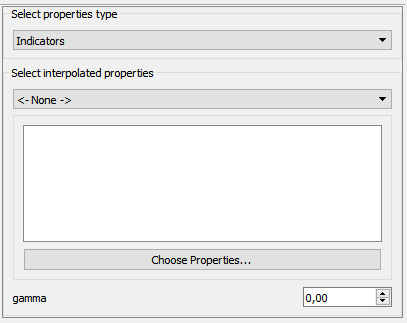
\includegraphics[width=0.6\textwidth]{apendice/imagens/block_tr.PNG}
\end{figure}

\section{Auxiliares}

Há ferramentas, que embora não sejam para modelagem geológica, auxiliam no processo de modelagem e visualização dos resultados.

\subsection{Criação automática do \textit{grid}}

O \textit{plugin} \textit{auto\underline{ }grid} (\autoref{autogrid}) cria um \textit{grid} que cobre toda área ou volume ocupado pelas amostras com dimensões dos blocos (sx, sy, sz) informadas pelo usuário. O parâmtro \textit{buffer} controla a extensão do \textit{grid} para além dos limites mínimos e máximos das amostras.

\begin{figure}[H]
	\caption{\label{autogrid}Interface do \textit{plugin} \textit{auto\underline{ }grid}}
	\centering
		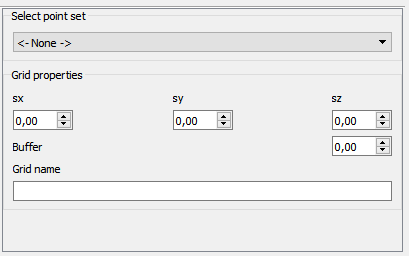
\includegraphics[width=0.6\textwidth]{apendice/imagens/autogrid.PNG}
\end{figure}

\subsection{Exportação em formato VTK}

O \textit{plugin} \textit{vtk\underline{ }export} (\autoref{vtk}) esporta propriedades em suporte de ponto ou bloco em formato VTK para visualização em outros softwares, como o Paraview, por exemplo.

\begin{figure}[H]
	\caption{\label{vtk}Interface do \textit{plugin} \textit{vtk\underline{ }export}}
	\centering
		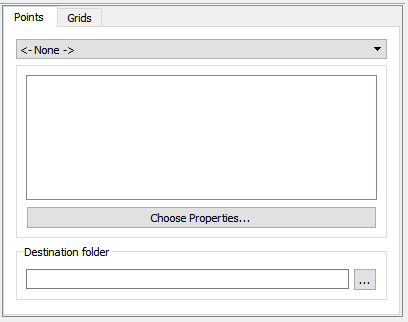
\includegraphics[width=0.6\textwidth]{apendice/imagens/vtk_export_1.PNG}
\end{figure}

\section{Modelagem determinística}

O \textit{plugin} \textit{deterministic} (\autoref{deterministic}) cria modelos geológicos uni ou multi categóricos a partir de distâncias assinaladas ou indicadores. Na aba \textit{general} (Figura \autoref{general}) O usuário seleciona se as propriedades são distâncias assinaladas ou indicadores. Deve selecionar o grid e o nome da propriedade que será criada. A opção \textit{keep all variables} cria, além do modelo final, todas as propriedades distâncias ou indicadores interpolados.

Se apenas uma categoria de distâncias assinaladas for escolhida a iso-superfície zero é extraída, se uma propriedade de indicadores for selecionada a abordagem apresentada na \autoref{problemas} é aplicada.
 
As propriedades interpoladas devem ser selecionadas em qualquer ordem, desde que tenham sido gradas pelo \textit{plugin} \textit{point\underline{ }transform} (\autoref{pttrans_sec}).

Em \textit{refinment options} O usuário insere os parâmetros para o refinamento de contatos (\autoref{bound_ref}): quantas iterações, zero gera um modelo sem refinamento, e os parâmetros de \textit{downscaling} do \textit{grid}, ou seja, em quantas partes as células serão divididas em x, y, e z.

Na aba \textit{variogram} o usuário insere os variogramas na mesma ordem que selecionou as variáveis interpoladas na aba anterior. Caso o usuário selecione a opção \textit{use variograms model file instead} ele deve carregar um arquivo de texto, como mostrado na \autoref{vario_model_txt}. O arquivo deve conter o número que representa cada categoria acompanhado do modelo variográfico em formato .xml, o mesmo formato usado pela ferramenta de variografia do \textit{AR2GemS}.

Caso um único variograma seja informado todas as categorias serão interpoladas com esse mesmo modelo. Caso nenhum variograma seja informado um modelo Gaussiano com um range igual a maior distância entre uma amostra codificada com aquele indicador e um nó do \textit{grid} é usado para cada uma das propriedades interpoladas selecionadas.

\begin{figure}[H] 
    \centering
    \caption{Interface do \textit{plugin} \textit{deterministic}} \label{deterministic}
     \subfloat[][Aba \textit{general}.]{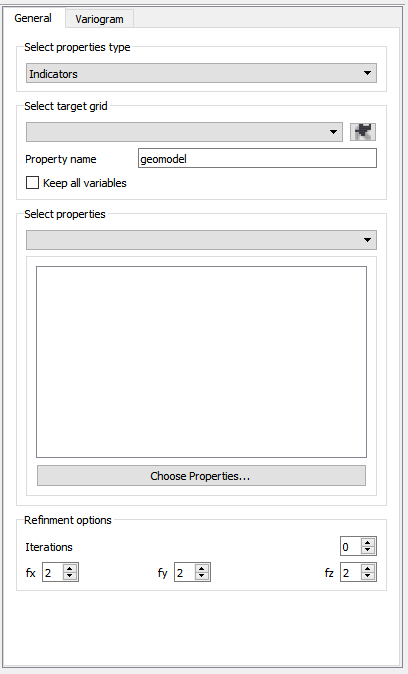
\includegraphics[width=.45\textwidth]{apendice/imagens/deterministic1.PNG}\label{general}}
     \hspace{1em}
     \subfloat[][Aba \textit{variogram}.]{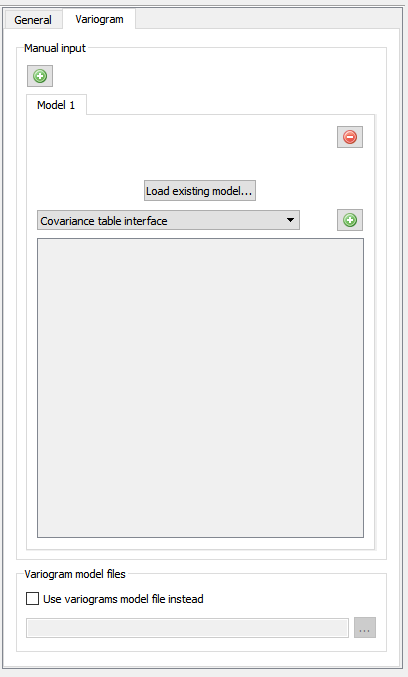
\includegraphics[width=.45\textwidth]{apendice/imagens/deterministic2.PNG}\label{variogram}}
\end{figure}

\begin{figure}[H]
	\caption{\label{vario_model_txt}Arquivo de texto com os modelos variográficos.}
	\centering
		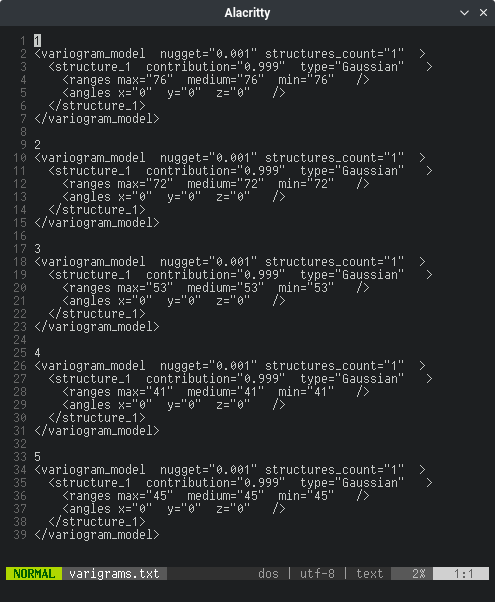
\includegraphics[width=0.6\textwidth]{apendice/imagens/variograms.png}
\end{figure}

\subsection{Máquina de vetores de suporte (SVM)}

A metodologia proposta por \citeonline{smirnoff2008support}, que usa máquina de vetores de suporte (\textit{support vector machine}) para a criação de modelos geológicos determinísticos multi-categóricos, foi implementada na suite.

\begin{figure}[H] 
    \centering
    \caption{Interface do \textit{plugin} \textit{svm}} \label{desvant}
     \subfloat[][Aba \textit{general}.]{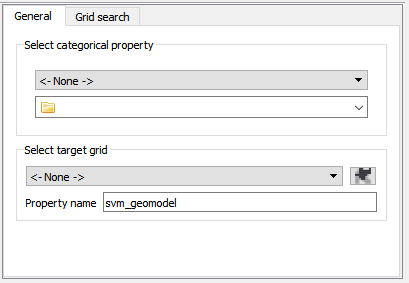
\includegraphics[width=.45\textwidth]{apendice/imagens/svm1.PNG}\label{<figure1>}}
     \hspace{1em}
     \subfloat[][Aba \textit{grid search}.]{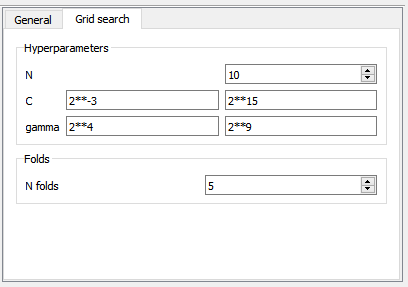
\includegraphics[width=.45\textwidth]{apendice/imagens/svm2.PNG}\label{<figure2>}}
\end{figure}

\begin{figure}[H]
	\centering
	\caption{\label{svm_model}Modelo geológico para o dataset \textit{Swiss Jura} criado com máquina de vetores de suporte.}
	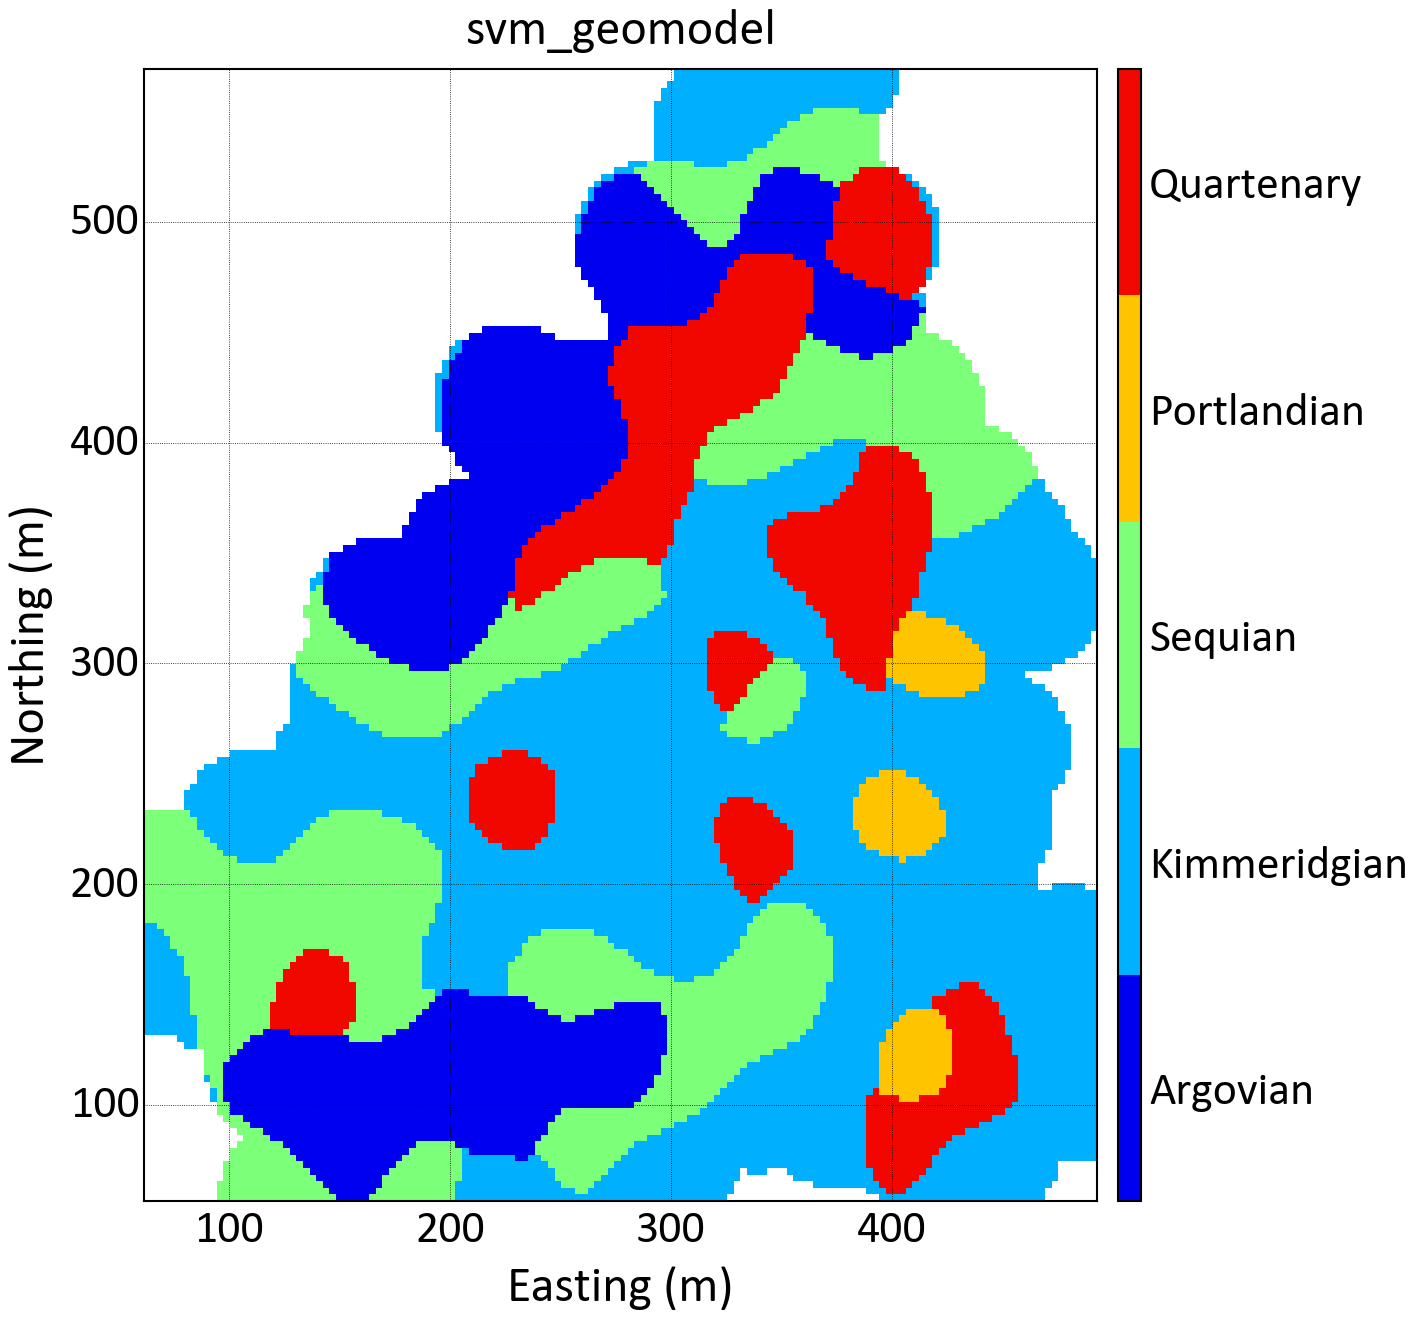
\includegraphics[width=0.6\textwidth]{apendice/imagens/svmgeomodel.png}
\end{figure}

\section{Modelagem estocástica}

\subsection{Parametrização do \textit{kernel}}

\begin{figure}[H] 
    \centering
    \caption{Interface do \textit{plugin} \textit{kernel\underline{ }factor\underline{ }uncertainty}.} \label{desvant}
     \subfloat[][Aba \textit{general}.]{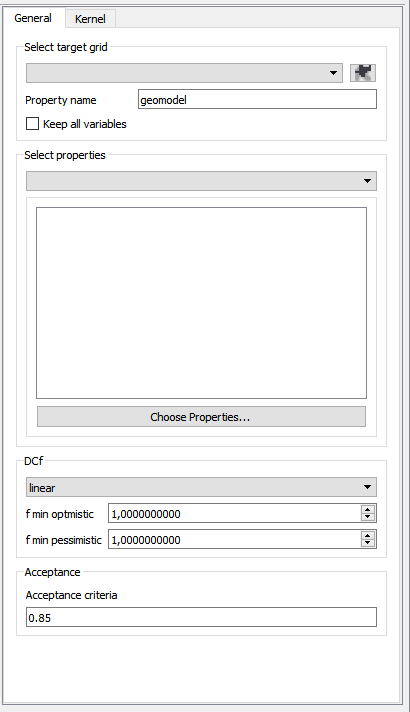
\includegraphics[width=.45\textwidth]{apendice/imagens/kf1.PNG}\label{<figure1>}}
     \hspace{1em}
     \subfloat[][Aba \textit{kernel}.]{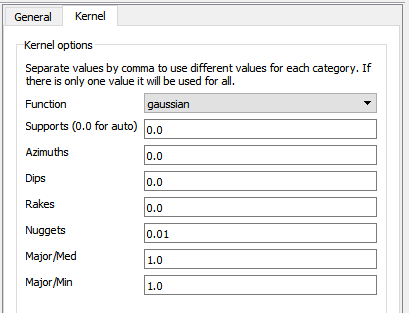
\includegraphics[width=.45\textwidth]{apendice/imagens/kf2.PNG}\label{<figure2>}}
\end{figure}

\subsection{Avaliação de incerteza usando funções distâncias assinaladas e campos potenciais}

\begin{figure}[H] 
    \centering
    \caption{Interface do \textit{plugin} \textit{boundary\underline{ }simulation\underline{ }pfields}.} \label{desvant}
     \subfloat[][Situação ideal, sem viés.]{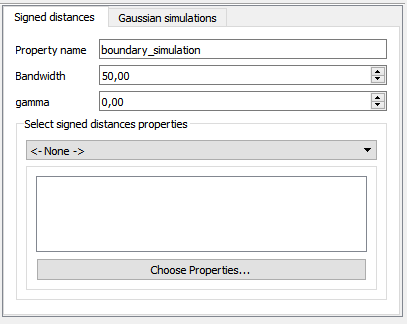
\includegraphics[width=.45\textwidth]{apendice/imagens/bound_sim_pfields1.PNG}\label{<figure1>}}
     \hspace{1em}
     \subfloat[][Situação real, com viés conservador.]{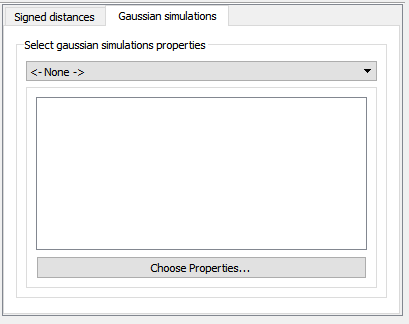
\includegraphics[width=.45\textwidth]{apendice/imagens/bound_sim_pfields2.PNG}\label{<figure2>}}
\end{figure}

\subsection{Simulação de contatos hierárquica}

















